%%%%%%%%%%%%%%%%%%%%%%% CHAPTER - 2 %%%%%%%%%%%%%%%%%%%%%%%%%%
\chapter{Fundamentals and Theoretical Framework of Neutrino Oscillations}
\label{C2} 
%%%%%%%%%%%%%%%%%%%%%%%%%%%%%%%%%%%%%%%%%%%%%%%%%%%%%%%%%%%%%%
%%%%%%%%%%%%%%%%%%%%%%%%%%%%
Neutrino oscillation is one of the pioneering discoveries in the history of particle physics. It has opened a new horizon for the community to utilize this second most abundant particle to reveal several mysteries of the Universe \cite{Tamborra:2024fcd}. The cornerstone of the neutrino oscillation was first laid in the Super-Kamiokande detector (Japan) in 1998 \cite{Super-Kamiokande:1998kpq} by providing experimental evidence in their data. Non-zero neutrino mass is the first experimental proof of BSM physics, for which the Nobel Prize was awarded to Takaaki Kajita and Arthur McDonald in 2015 \cite{Kajita:2016cak, McDonald:2016ixn}.\\
Before entering into the formalism of neutrino oscillation, it is essential to know why neutrinos show the flavor transition (named ``neutrino oscillation") \cite{Rajasekaran:2000nn, Agarwalla:2008jin}, whereas their charged counterparts do not show oscillations. Neutrino oscillation is a mass-induced phenomenon. Due to the non-zero value of neutrino mass and the non-degenerate values of the mass eigenstates \cite{Raychaudhuri:2000zn}, the flavor eigenstates and mass eigenstates of neutrinos are quite different. The tiny mass-squared differences between the neutrino mass eigenstates ($\sim 10^{-5}$ to $10^{-3} \, \mathrm{eV}^2$) protect the coherence of the superposition \cite{LIPKIN2004355, Ravari:2022yfd} of mass eigenstates to the flavor states. In contrast, the mass differences between the leptons are so huge ($\sim 100$ MeV to GeV scale) that any superposition of the mass eigenstates of the leptons decoheres almost immediately before their significant propagation.\\
This chapter is planned in the following way. Section \ref{sec:2.1} outlines the fundamental theoretical framework of neutrino oscillations in the vacuum, examining the formalism in the two-flavor framework. In section \ref{sec:2.2}, the extension of this formalism in the three-flavor landscape is described. In section \ref{sec:2.3}, we introduce matter-effect in our discussion, incorporating standard neutrino-matter interactions within both two-flavor and three-flavor scenarios. Section \ref{sec:2.4} provides an overview of several relevant neutrino oscillation experiments and their contributions to measuring oscillation parameters. In section \ref{sec:2.4}, we present the current status of the six oscillation parameters and the so-called eight-fold degeneracies, discussing their experimental determination. Finally, in section \ref{sec:2.5}, we provide a concluding overview of this chapter.\\

\section{The mathematical framework of two-flavor neutrino oscillation}
\label{sec:2.1}
There are several approaches to construct the neutrino oscillation framework. Neutrinos are fermions and occupy their places in the lepton family of the SM, in the form of $SU(2)$ doublets. So, ideally, the Dirac equation should lead us to the neutrino oscillation probability. However, neutrino oscillation does not manifest any spin nature of itself, and hence, for the ease of our calculations, we use the Schr\"{o}dinger equation considering neutrino as a free particle instead of assuming it as a wave packet. Neutrinos are produced or detected at their flavor eigenstates ($\nu_e$, $\nu_\mu$, or $\nu_\tau$) or weak eigenstates (or gauge states), but they are in the mass eigenstates or physical states ($\nu_1$ and $\nu_2$) while propagating through the vacuum or the matter. The mass eigenstates and flavor eigenstates are considered to form a complete orthonormal basis to conserve the flavor transition probability, and hence a flavor eigenstate, $\nu_\alpha$ is connected to the mass eigenstate $\nu_k$ through a unitary matrix $U$ in the following fashion.

\begin{align}
\ket{\nu_{\alpha}}=\sum_{k=1}^{2}U_{\alpha k}\ket{\nu_{k}},
\end{align}
where $\alpha$ is the flavor index [$\alpha$ = \{$e$, $\mu$\}, or \{$e, \tau$\}, or \{$\mu, \tau$\}] and k is the mass index, $U_{\alpha k}$ are the elements of the unitary matrix connecting the bridge between this two orthonormal basis, ensuring the probability conservation. The completeness of the basis indicates that $\sum_{\alpha} \ket{\nu_\alpha}\bra{\nu_\alpha} = \sum_{k=1,2} \ket{\nu_k}\bra{\nu_k}=\mathds{1}$, whereas the orthonormality ensures that $ \langle \nu_\alpha | \nu_\beta \rangle = \delta_{\alpha \beta}$  and 
 $ \langle \nu_i | \nu_j \rangle=  \delta_{ij}$. The crucial point is to be noted here that the three mass eigenstates are non-degenerate ($i.e.$, the mass of each eigenstate must not be equal, $m_1\neq m_2$, where $m_k$ is the mass of the eigenstate $\nu_k$). These mass eigenstates evolve with time while neutrinos propagate through the vacuum or the matter, and hence, the flavor eigenstates are also affected by time evolution. As the mass eigenstates are the eigenstates of the Hamiltonian, we can write the time evolution of the mass eigenstates in the following way.\\
\par Let us consider a system where a neutrino beam of flavor state $\ket{\nu_{\alpha}(0,0)}$ is generated at space-time point $(x,t)=(0,0)$.\\
We know while the neutrino will propagate through the vacuum they are in mass eigenstates and its time evolution will be governed by the time-dependent Schr\"{o}dinger equation, $i.e.$,\\
\begin{align}
i\frac{\partial}{\partial t}\ket{\nu_{k}(x,t)}&=E\ket{\nu_{k}(x,t)}\\
&=\frac{-1}{2m_{k}}\frac{\partial^2}{\partial^2 x}\ket{\nu_{i}(x,t)},
\end{align}
	where, $k=1,2$. Here, we have used the natural units ($i.e.$, $\hbar$=1).\\
	Now, 
	\begin{align}
	i\frac{\partial}{\partial t}\ket{\nu_{k}(x,t)}&=E\ket{\nu_{k}(x,t)}\\
	\Rightarrow&\frac{\partial\ket{\nu_{k}(x,t)}}{\ket{\nu_{k}(x,t)}}=-iE\partial t	.
	\end{align}\\
	Performing partial integration, we get \\
	\begin{align}
\ket{\nu_{k}(x,t)}=e^{-iE_{k}t}\ket{\nu_{i}(0,0)},
\end{align}
and the trial solution $\ket{\nu_{k}(x,t)}=e^{ip_{k} x}$ satisfies the equation\\
\begin{align}
\frac{-1}{2m_{k}}\frac{\partial^2}{\partial^2 x}\ket{\nu_{k}(x,t)}=E\ket{\nu_{k}(x,t)}.
\end{align}
So finally,\\
\begin{align}
\ket{\nu_{k}(x,t)}&=e^{-i(E_{k}t-p_{k}x)}\ket{\nu_{k}(0,0)}\\
&=e^{-i\phi_{k}}\ket{\nu_{k}(0,0)}, 
\end{align}
where,\\
\begin{equation}
 \phi_{k}=E_{k}t-p_{k}x.
 \label{equn:2.10}
 \end{equation}
At some later space-time point (x,t), the time evolved flavor state $\ket{\nu}_\alpha$ will be\\
\begin{align}
\ket{\nu_{\alpha}(x,t)} &=\sum_{k=1}^{2} U_{\alpha k}\ket{\nu_{k}(x,t)} \\
&=\sum_{k=1}^{2} U_{\alpha k} e^{-i\phi_{k}}\ket{\nu_{k}(0,0)} .
\label{eqn:2.12}
\end{align}
So,\\
\begin{align}
\ket{\nu_{k}(0,0)}=\sum_{\gamma}U^*_{\gamma k}\ket{\nu_{\gamma}(0,0)}. 
\label{eqn:2.13}
\end{align}
Here $\gamma$ is a dummy index of the unitary matrix while being inverted.\\
We have to find the evolution of flavor states, but from the Schr\"{o}dinger equation, we got the time evolution of mass eigenstates as they are the eigenstates of the governing Hamiltonian.\\
So, substituting equation \ref{eqn:2.13} into equation \ref{eqn:2.12}, we get,\\
\begin{align}
	\ket{\nu_{\alpha}(x,t)}&=\sum_{k=1}^{2}U_{\alpha k}e^{-i\phi_{k}}\sum_{\gamma=1}^{2}U^*_{\gamma k}\ket{\nu_{\gamma}(0,0)}\\
	&=\sum_{\gamma}\sum_{k}U^*_{\gamma k}e^{-i\phi_{k}}U_{\alpha k}\ket{\nu_{\gamma}(0,0)}.
\end{align}
Transition amplitude for detecting a neutrino of flavor $\beta$ at space-time point (t,x) when generation of a neutrino of flavor $\alpha$ at space-time point (0,0) is\\
\begin{align}
A(\ket{\nu_{\alpha}(0,0)}\rightarrow\nonumber \ket{\nu_{\beta}(x,t)})&=\braket{\nu_{\beta}(x,t)|\nu_{\alpha}(0,0)}\\\nonumber
 &=\sum_{\gamma}\sum_{k}U_{\gamma k}e^{i\phi_{k}}U^*_{\beta k}\braket{\nu_{\gamma}(0,0)|\nu_{\alpha}(0,0)}\\\nonumber
 &=\sum_{\gamma}\sum_{k}U_{\gamma k}e^{i\phi_{k}}U^*_{\beta k}\delta_{\gamma\alpha}\\
 &=\sum_{k}U_{\alpha k}e^{i\phi_{k}}U^*_{\beta k}.
\end{align}
So, the oscillation probability is,
\begin{align}
	P(\nu_{\beta}\rightarrow\nu_{\alpha})&=|A(\ket{\nu_{\beta}(0,0)}\rightarrow \nonumber\ket{\nu_{\alpha}(x,t)})|^2\\\nonumber
	&=|\sum_{k}U_{\alpha k}e^{i\phi_{k}}U^*_{\beta k}|^2\\ \nonumber
	&=\sum_{k}U_{\alpha k}e^{i\phi_{k}}U^*_{\beta k}\sum_{j}U^*_{\alpha j}e^{-i\phi_{j}}U_{\beta j}\\
	&=\sum_{j=1}^{2}\sum_{k=1}^{2}U_{\alpha k}U^*_{\beta k}U^*_{\alpha_j}U_{\beta j}e^{-i(\phi_{j}-\phi_{k})} .
    \label{equn:2.17}
\end{align}
For the two-flavor oscillation, the $(2\times2)$ unitary matrix is just a rotation matrix in 2d.\\
\begin{equation}
U= \begin{pmatrix}
 U_{\alpha_1} & U_{\alpha_2} \\
 U_{\beta_1} & U_{\beta_2} \\
\end{pmatrix}
=	\begin{pmatrix}
\cos\theta & \sin\theta\\
-\sin\theta & \cos\theta\\
	\end{pmatrix},
\end{equation}
where $\theta$ is a parameter called the mixing angle. For the two-flavor oscillation, it is the only mixing parameter as a $2\times2$ unitary matrix can be parameterized by only one parameter. We show the calculation of equation \ref{equn:2.17} term by term.\\
For \underline{\bf{$k=1,\,j=1;$}}\\
\begin{align}
P_1(\nu_{\beta}\rightarrow\nonumber\nu_{\alpha})&=U_{\alpha 1}U^*_{\beta 1}U^*_{\alpha_1}U_{\beta 1}e^{-i(\phi_{1}-\phi_{1})}\\
&=|U_{\beta 1}|^2|U_{\alpha_1}|^2.
\end{align}
For \underline{\bf{$k=2,\,j=2;$}}\\
\begin{align}
P_2(\nu_{\beta}\rightarrow\nu_{\alpha})=|U_{\beta 2}|^2|U_{\alpha_2}|^2.
\end{align}
For \underline{\bf{$k=1,\,j=2;$}}\\
\begin{align}
P_3(\nu_{\beta}\rightarrow\nu_{\alpha})=U_{\alpha 1}U^*_{\beta 1}U^*_{\alpha 2}U_{\beta 2}e^{-i(\phi_{2}-\phi_{1})}.
\end{align}
For \underline{\bf{$k=2,\,j=1;$}}\\
\begin{align}
P_4(\nu_{\beta}\rightarrow\nu_{\alpha})=U_{\alpha 2}U^*_{\beta 2}U^*_{\alpha 1}U_{\beta 1}e^{-i(\phi_{1}-\phi_{2})}.
\end{align}
Finally, \\
\begin{align}
P(\nu_{\beta}\rightarrow\nonumber\nu_{\alpha})&=|U_{\beta 1}|^2|U_{\alpha 1}|^2+|U_{\beta 2}|^2|U_{\alpha 2}|^2+U_{\alpha 1}U^*_{\beta 1}U_{\alpha 2}U^*_{\beta 2}\left(e^{i\left(\phi_{2}-\phi_{1}\right)}+e^{-i\left(\phi_{2}-\phi_{1}\right)}\right)\\\nonumber
&=(\sin^2\theta\cos^2\theta+\cos^2\theta\sin^2\theta)+2\,U_{\alpha 1}U^*_{\beta 1}U_{\alpha 2}U^*_{\beta 2}\cos(\phi_{2}-\phi_{1})\\\nonumber
&=2\sin^2\theta\cos^2\theta+2\cos\theta(-\sin\theta)\sin\theta\cos\theta\cos(\phi_{2}-\phi_{1})\\\nonumber
&=2\sin^2\theta\cos^2\theta\,[1-\cos(\phi_{2}-\phi_{1})]\\\nonumber
&=4\sin^2\theta\cos^2\theta\sin^2\left(\frac{\phi_{2}-\phi_{1}}{2}\right)\\\nonumber
&=\sin^2(2\theta)\sin^2\left(\frac{\phi_{2}-\phi_{1}}{2}\right).\\
\label{equn:2.23}
\end{align}
By equation \ref{equn:2.10},
\begin{align}
\phi_{k}=E_{k}t-p_{k}x.
\end{align}
So,
\begin{align}
\phi_{2}-\phi_{1}=(E_2-E_1)t-(p_2-p_1)x.
\end{align}
\textit{At this point, we make our first assumption that neutrinos are relativistic}, so $t=x=L$. Here, $L$ is the length of the baseline, and $E$ is the true neutrino energy. As we are in natural unit scale, $c=1$, and 
\begin{align}
p_i&=\nonumber\sqrt{E^2_i-m^2_i}\\\nonumber
&=E_i\sqrt{1-\frac{m^2_i}{E^2_i}}\\\nonumber
&\approx E_i(1-\frac{m^2_i}{2E^2_i})\\\nonumber
&=E_{i}-\frac{m^2_i}{2E_i},\\
\label{equn:2.26}
\end{align}
as neutrino masses are very small compared to their energy.\\
By equation \ref{equn:2.26},\\
\begin{align}
 \phi_{2}-\phi_{1}=\left(\frac{m^2_2}{2E_2}-\frac{m^2_1}{2E_1}\right)L.
 \end{align}
 \textit{Our next assumption posits that each neutrino flavor state is associated with a well-defined momentum p, implying that all mass eigenstates $\nu_i$ (i= 1,2) possess an identical momentum. This premise is grounded in the notion that all mass eigenstates emanate from a common source and traverse coherently along the same trajectory.} It is to be noted here that mass eigenstates are assumed as plane wave solutions. Henceforth, we will consider $E_1=E_2=E$ in our calculation.\\
 Now,\\
 \begin{align}
 \phi_{2}-\phi_{1}&=\nonumber\left(\frac{m^2_2}{2E}-\frac{m^2_1}{2E}\right)\,L\\
 &=\frac{\Delta m^2\,L}{2E},
 \end{align}
 where, $\Delta m^2=m^2_2-m^2_1$.\\
 By equation \ref{equn:2.23}, we can write the probability of the neutrino oscillation from the flavor $\alpha$ to the flavor $\beta$ is \\
 \begin{align}
 P(\nu_{\alpha}\rightarrow\nu_{\beta})=\sin^2\left(2\theta\right)\sin^2\left(\frac{\Delta m^{2}\,L}{4E}\right).
 \label{eq:2-flavor vacuum oscillation formula}
 \end{align}
 \par Here, the first term signifies the amplitude part of the oscillation (governed by the parameter ``mixing angle" $\theta$), and the second term signifies the frequency part (governed by the parameter ``mass-squared difference" $\Delta m^2$). They are fixed in Nature. Here, we have calculated the oscillation probability by imposing natural units ($i.e.$, $\hbar$=c=1).\\
 \par  Now, if we want this oscillation probability formula compatible with the data obtained from the experiments, we need to convert the units of the equation \ref{eq:2-flavor vacuum oscillation formula} $\left[\Delta m^2\, (\mathrm{in \,\,eV}^2), \, L \,(\mathrm{in\,\, eV}^{-1}),\, E\, (\mathrm{in\,\, eV})\right]$ to the units used by the experiments [$i.e.$, $\Delta m^2\, (\mathrm{in\,\,eV}^2), \, L \,(\mathrm{in \,\,km}),\, E\, (\mathrm{in\,\,GeV})$]. The quantity  $\left(\dfrac{\Delta m^2\, L}{4E}\right)$ is in the argument of a sinusoidal function and needs to be dimensionless. After implementing those conversion factors, the final form of the neutrino oscillation probability from a flavor $\alpha$ to be transited to a flavor $\beta$ through vacuum in the two-flavor landscape is,
 \begin{align}
P(\nu_{\alpha}\rightarrow\nu_{\beta})=\sin^2\left(2\theta\right)\sin^2\left(1.27\times\frac{\Delta m^{2}\,L}{E}\right),
\label{eq:2 flavor app oscillation probability}
 \end{align}
where $L$ is the length over which neutrino changes its flavor (in km), E is the true neutrino energy (in GeV), and $\Delta m^2_{21}$ is the mass-squared difference (in $\mathrm{eV}^2$), where $\Delta m^2= m^2_2-m^2_1$. It is noteworthy that, two flavor neutrino oscillation only suggests the non-trivial mixing and mass-induced flavor conversion in the neutrino sector but cannot predict anything regarding the CP violation. 
Similarly, the expression of the survival (or disappearance) probability in the two-flavor landscape can be written as,
\begin{align}
P(\nu_{\alpha}\rightarrow\nu_{\alpha})=1-\sin^2\left(2\theta\right)\sin^2\left(1.27\times\frac{\Delta m^{2}\,L}{E}\right).
\label{eq:2 flavor oscillation probability}
 \end{align}

 %----------------------------------------------------------
\begin{figure}[htb!]
	\centering
	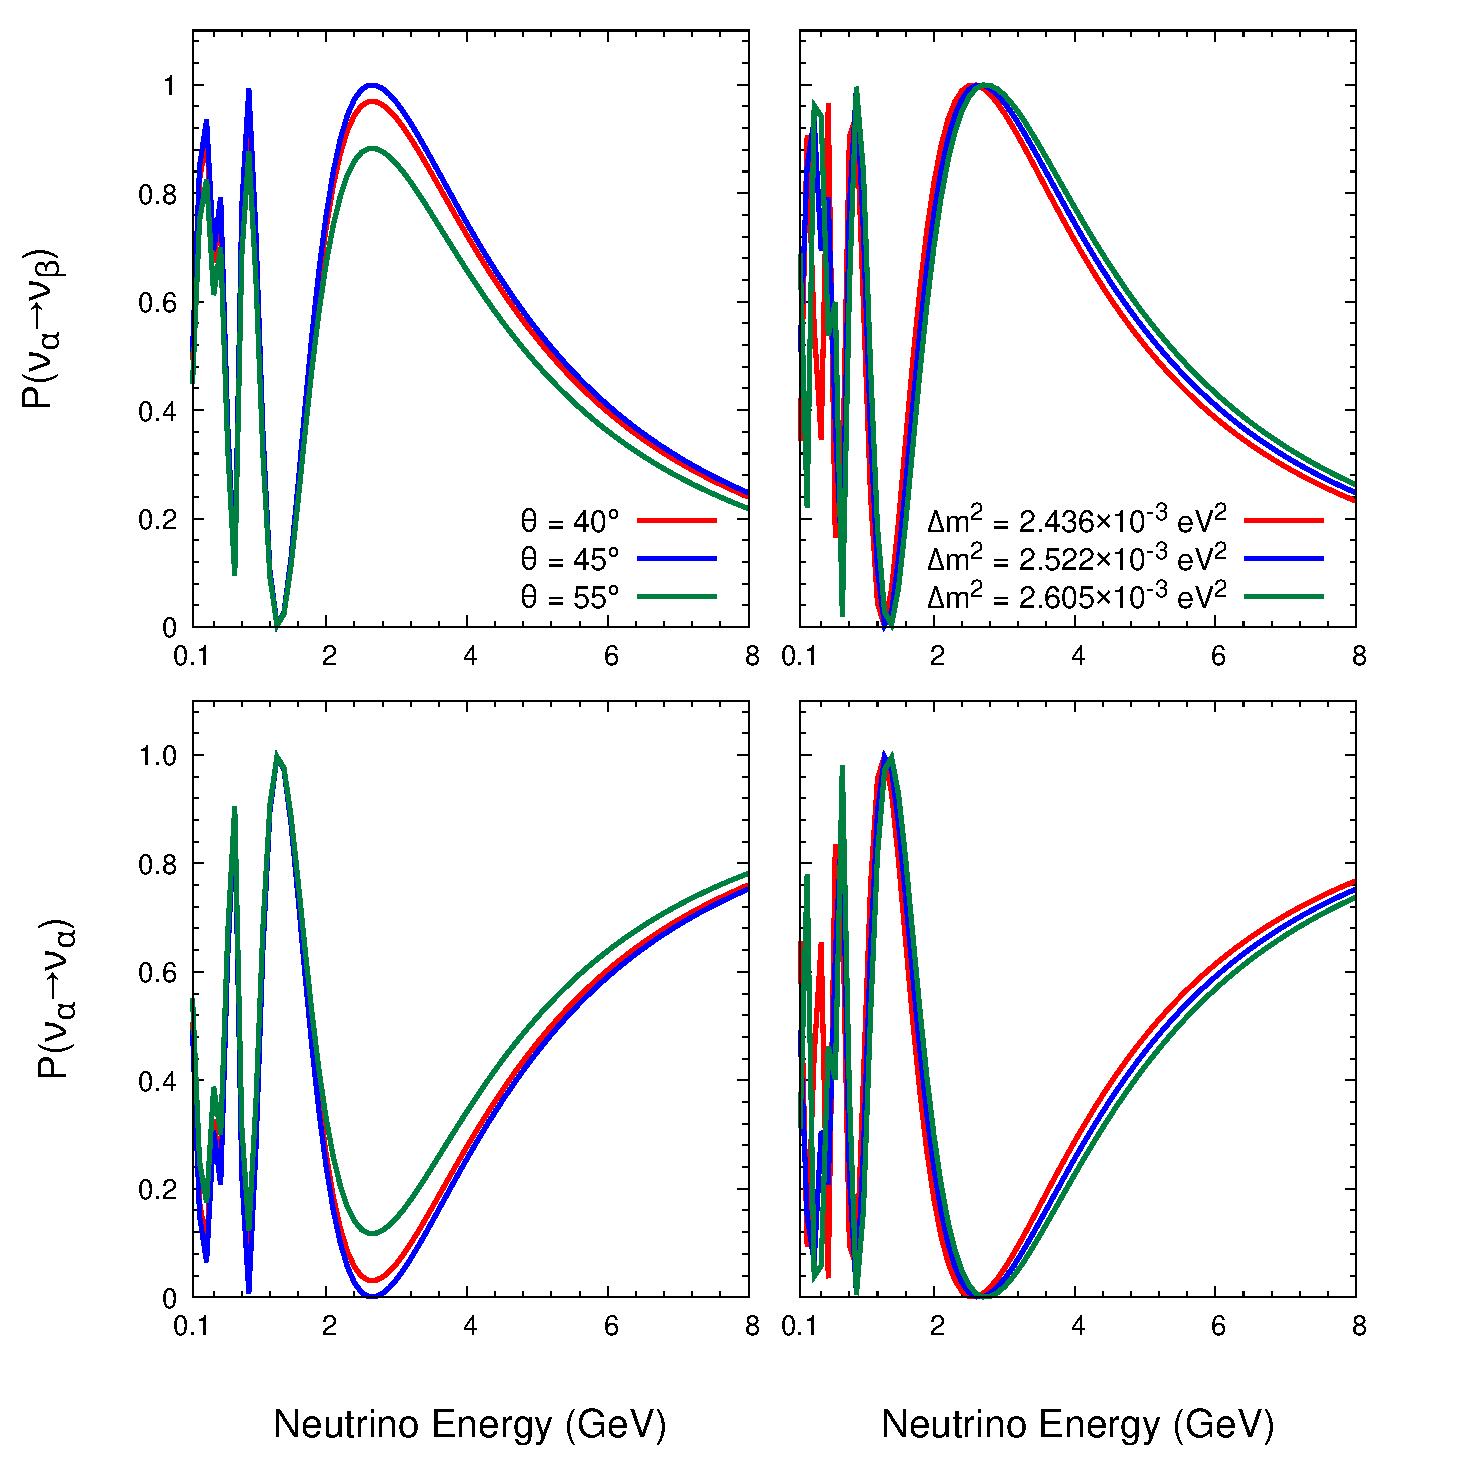
\includegraphics[width=\linewidth]{./Figures/Chapter-2/Thesis_multiplot_prob_app_disapp.pdf}	
    \caption{\footnotesize{Neutrino oscillation probability in vacuum at two flavor case as the function of true neutrino energy (in GeV) is depicted here. The upper (lower) panel represents $\nu_\alpha\rightarrow\nu_\beta$ appearance ($\nu_\alpha\rightarrow\nu_\alpha$ disappearance) probability using Equation \ref{eq:2 flavor app oscillation probability}. In the left panel, we observe the oscillation probability for three choices of mixing angle $\theta\,\,i.e.,\,\,40^\circ,\,45^\circ,\,\mathrm{and}\,\,\, 55^\circ$ (shown in red, blue, and green lines), respectively, assuming $L= 1300$ km and $\Delta m^2=+2.522\times10^{-3}$ eV$^2$. In the right panel, we compute the same but for three different choices of $\Delta m^2,\,\,i.e.,\,2.436\times10^{-3}$ eV$^2,\, 2.522\times10^{-3}$ eV$^2, \mathrm{and}\,\,\, 2.605\times10^{-3}$ eV$^2$ (shown by red, blue, and green lines), respectively, assuming a given mixing angle $\theta=45^\circ$.}}
	\label{fig:oscillation_prob_vacuum_analytical}
\end{figure} 
%------------------------------------
 \par Equation \ref{eq:2 flavor app oscillation probability} resembles with the standard oscillation formula in the acoustic medium, where the first part signifies the amplitude part (governed by the mixing angle $\theta$), whereas the second part depicts the frequency part (governed by the mass-squared difference $\Delta m^2$). If $\theta$ becomes $45^\circ$, appearance probability (\ref{eq:2 flavor app oscillation probability}) becomes maximum. Hence the value $\theta=45^\circ$ is called the maximal mixing (MM) value \cite{Xing:2015fdg}. Any other values of $\theta$ show lesser appearance probability than the maximal mixing for a given set of values of oscillation parameters. On the other hand, the shift of the frequency can be tuned to different energy and baseline lengths by controlling the value of $\Delta m^2$. 

 Figure~\ref{fig:oscillation_prob_vacuum_analytical} illustrates that the variations in the mixing angle enable precise modulation of the amplitude of the neutrino oscillation probability, while adjustments to the mass-squared difference primarily govern the phase shift of the oscillation pattern. The mixing angle $\theta$ signifies the extent of flavor mixing, with maximal mixing corresponding to the highest transition probability or the deepest suppression in survival probability. Moreover, in the oscillation frequency domain, an increase in the value of $\Delta m^2$ induces a phase shift toward higher neutrino energies, resulting in a rightward displacement of the oscillation peak.\\
 %-----------------------------------------------------
 \section{Formalism of neutrino oscillation probability in $3\nu$ paradigm}
 \label{sec:2.2}
 The discovery of the non-zero value of $\theta_{13}$ in the Daya Bay \cite{DayaBay:2012fng, DayaBay:2022orm} experiment connects the atmospheric neutrino sector and the solar neutrino sector, establishing the $3\nu$ paradigm on a strong footing. At the same time, the two-flavor neutrino oscillation delineates the values of the solar and atmospheric oscillation parameters, and the $3\nu$ paradigm with non-zero $\theta_{13}$ gives rise to the possibilities of observing CP violation in the neutrino sector. Now, we discuss the formalism of the three-flavor neutrino oscillation.
 \par Let, a neutrino of flavor $ \alpha$ is produced at $ x=0 $ with energy $E$, then the state of the neutrino at $x=0$ can be expressed as\\
 	\begin{align}
 		\ket{\nu_{\alpha}(x=0)}& =\nonumber\ket{\nu_\alpha}\\
 		&=\sum_{j=1}^{3}(U_{PMNS})^*_{\alpha j}\ket{\nu_j}.\\\nonumber
  	 	\end{align}
 At the position $x=L$, the neutrino state can be written as,\\
 \begin{align}
 	\ket{\nu_{\alpha}(x=L)}&=\nonumber\sum_{j=1}^{3}e^{ip_jL}(U_{PMNS})^*_{\alpha j}\ket{\nu_j}\\
 	&=e^{ip_kL}\sum_{j=1}^{3}e^{i(p_j-p_k)L}(U_{PMNS})^*_{\alpha j}\ket{\nu_j}.\\\nonumber
 \end{align}
   	
   	Assuming $m_j<<E$ we can approximate, \\
   	\begin{align}
   		p_j&=\nonumber\sqrt{E^2-m^2_j}\\
   		&=E-\frac{m^2_j}{2E}+...\\\nonumber.
   	\end{align}
   So,
   \begin{align}
   	p_j-p_k \approx -\frac{\Delta m^2_{jk}}{2E}\\\nonumber
   \end{align}
   where, $\Delta m^2_{jk}=m^2_j-m^2_k$ . \\
   	 %  	\newpage
   	   	Hence, we can write
   	   	\begin{align}
   	   		\ket{\nu_{\alpha}(x=L)}&=e^{ip_kL}\sum_{j=1}^{3}exp\left(-i\frac{\Delta m^2_{jk}\,L}{2E}\right)(U_{PMNS})^*_{\alpha j} \ket{\nu_j}.\\\nonumber
   	   	\end{align}
   	   	%\newpage
        \vspace{-1.5mm}
   	So, the probability amplitude of observing the neutrino flavor $\beta$ at $x=L$ is given by (neglecting the overall phase as it will be cancelled out while multiplying with its complex conjugate while obtaining the probability),   
	\begin{align}
  	\textrm{A}_{\beta\alpha}&=\nonumber\braket{{\nu_\beta}|\nu_{\alpha}(x=L)}\\\nonumber
	&=\nonumber\left[\sum_{k=1}^{3}\bra{\nu_k}(U_{PMNS})_{\beta k}\right]\left[\sum_{j=1}^{3}\exp\left(-i\frac{\Delta m^2_{jk}\,L}{2E}\right)(U_{PMNS})^*_{\alpha j}\ket{\nu_j}\right]\\\nonumber
   	&=\nonumber\sum_{j=1}^{3}(U_{PMNS})_{\beta j}\exp\left(-i\frac{\Delta m^2_{jk}\,L}{2E}\right)(U_{PMNS})^*_{\alpha j}\\
   	&=\sum_{j=1}^{3}U_{\beta j}\exp\left(-i\frac{\Delta m^2_{jk}\,L}{2E}\right)U^*_{\alpha j}.\\\nonumber
  	\end{align}	
  	So, the probability of oscillation from $\ket{\nu_\alpha}$ to $\ket{\nu_\beta}$ with true neutrino energy $E$ and baseline $L$ is given by,\\
  	\begin{align}
  		P(\nu_\alpha \rightarrow \nu_\beta)&=\nonumber|A_{\beta\alpha}|^2\\\nonumber
  		&=\nonumber|\sum_{j=1}^{3}U_{\beta j}exp\left(-i\frac{\Delta m^2_{jk}\,L}{2E}\right)U^*_{\alpha j}|^2\\\nonumber
  		&=\nonumber \left[\sum_{j=1}^{3}U_{\beta j}exp\left(-i\frac{\Delta m^2_{jk}\,L}{2E}\right)U^*_{\alpha j}\right]\times\left[\sum_{i=1}^{3}U_{\alpha i}exp\left(i\frac{\Delta m^2_{ik}\,L}{2E}\right)U^*_{\beta i}\right]\\
  		&=\sum_{j=1}^{3}\sum_{i=1}^{3}exp\left[-i\frac{\left(\Delta m^2_{jk}-\Delta m^2_{ik}\right)\,L}{2E}\right]\,U_{\beta j}U^*_{\alpha j}U_{\alpha i}U^*_{\beta i}\\\nonumber
  		\label{Equation 8}\\
  		&=\sum_{i}\sum_{j}\left(A_{ij}+iB_{ij}\right)\times\left(C_{ij}+iD_{ij}\right);    (say),\\\nonumber
  	\end{align}
   	   	where we assume, $exp\left[-i\dfrac{\left(\Delta m^2_{jk}-\Delta m^2_{ik}\right)\,L}{2E}\right]=A_{ij}+iB_{ij}$ and $U_{\beta j}U^*_{\alpha j}U_{\alpha i}U^*_{\beta i}=C_{ij}+iD_{ij}$. As the oscillation probability is a measurable quantity, so it should be real. Hence, we can drop the imaginary component of equation \ref{Equation 8}.\\
        
   	   	We break the sum of equation \ref{Equation 8} in two parts, $i.e.,$\\
   	   	\[
\sum_{i=1}^{3} \sum_{j=1}^{3} = \sum_{\substack{i=j=1}}^{3} + \sum_{\substack{i \neq j \\ i=1,\, j=1}}^{3}.
\]        
   	   	\textbf{\underline{Case - 1 :}}\\
   	   	for $i=j$,\\
   	  \begin{align}
   	  	 exp\left[-i\frac{\Delta m^2_{ii}\,L}{2E}\right]U_{\beta i}U^*_{\alpha i}U_{\alpha i}U^*_{\beta i}	&= U_{\beta i}U^*_{\alpha i}U_{\alpha i}U^*_{\beta i}.\\\nonumber
   	  \end{align}
   	   	\textbf{\underline{Case - 2 :}}\\
   	   for $i\neq j$,\\
   	   \begin{align}
   	   Re\left(exp\left[-i\frac{\Delta m^2_{ji}\,L}{2E}\right]\right)&=\nonumber \cos\left(\frac{\Delta m^2_{ji}\,L}{2E}\right)\\
   	   &=\cos(\Delta_{ji});\,\,(say, A_{ij}),\\
   	   Im\left(exp\left[-i\frac{\Delta m^2_{ji}\,L}{2E}\right]\right)&=\nonumber -\sin\left(\frac{\Delta m^2_{ji}\,L}{2E}\right)\\
   	   &=-\sin(\Delta_{ji});\,\,(say, B_{ij}).\\\nonumber
   	   \end{align}	
   	   	So, from equation \ref{Equation 8}, considering the real part only, we can write\\
   	   	\begin{align}
    P (\nu_\alpha \rightarrow \nu_\beta) &= A_{ij}C_{ij} - B_{ij}D_{ij} \nonumber \\
    &= Re (U^*_{\alpha i} U_{\beta i}U_{\alpha j}U^*_{\beta j}) 
    - 2\,Re (U^*_{\alpha i} U_{\beta i}U_{\alpha j}U^*_{\beta j}) \sin^2\left(\frac{\Delta_{ji}}{2}\right) \nonumber \\
    &\quad + Im\,(U^*_{\alpha i} U_{\beta i}U_{\alpha j}U^*_{\beta j}) \sin(\Delta_{ji}). \label{Equation12}
\end{align}
	   	Here, we have used $\cos(\Delta_{ji})=1-2\sin^2\left(\dfrac{\Delta_{ji}}{2}\right)$. So, taking case - 1 ($i.e.$, $i=j$) and case - 2 ($i\neq j$) together, we can write,
  \begin{align}
    P(\nu_\alpha \rightarrow \nu_\beta) &= \sum_{i}\sum_{j} \Big[ U_{\beta i}U^*_{\alpha i}U_{\alpha i}U^*_{\beta i} 
    + Re\,(U^*_{\alpha i} U_{\beta i}U_{\alpha j}U^*_{\beta j}) \nonumber \\
    &\quad - 2Re\,(U^*_{\alpha i} U_{\beta i}U_{\alpha j}U^*_{\beta j}) \sin^2\left(\frac{\Delta_{ji}}{2}\right) \nonumber \\
    &\quad + Im\,(U^*_{\alpha i} U_{\beta i}U_{\alpha j}U^*_{\beta j}) \sin(\Delta_{ji}) \Big]. \label{Equation}
\end{align}
  Now,
\begin{align}
    \left(\sum_{i=1}^{3}U^*_{\alpha i}U_{\beta i}\right)^2 &= 
    \left(U^*_{\alpha 1}U_{\beta 1} + U^*_{\alpha 2}U_{\beta 2} + U^*_{\alpha 3}U_{\beta 3} \right)^2 \nonumber \\
    &= \sum_{i}(U^*_{\alpha i}U_{\beta i})^2 + \sum_{i \neq j} 2(U^*_{\alpha i} U_{\beta i}U_{\alpha j}U^*_{\beta j}). \label{Equation13}
\end{align}
   So, from the equation \ref{Equation13}, we can write the final generalized form of the equation of neutrino oscillation probability in $3\nu$ framework as \\
   \begin{align}
    P(\nu_\alpha \rightarrow \nu_\beta) &= \delta_{\alpha\beta} 
    - 4\sum_{i>j} Re\,(U^*_{\alpha i} U_{\beta i}U_{\alpha j}U^*_{\beta j}) \sin^2\left(\frac{\Delta_{ji}}{2}\right) \nonumber \\
    &\quad + 2\sum_{i>j} Im\,(U^*_{\alpha i} U_{\beta i}U_{\alpha j}U^*_{\beta j}) \sin(\Delta_{ji}). \label{Equation14}
\end{align}
If $i$ and $j$ take only values from 1 to 2, the above equation reduces to the two-flavor neutrino oscillation expression. The third term of equation \ref{Equation14} represents the CP violation. The PMNS matrix can be written as,
\begin{equation}
   	  U= 
   	   \begin{pmatrix}
	1 & 0 & 0 \\
	0 & c_{23} & s_{23} \\
	0 & -s_{23} & c_{23}
\end{pmatrix} 
\begin{pmatrix}
	c_{13} & 0 & s_{13}e^{-i\delta} \\
	0 & 1 & 0 \\
	-s_{13}e^{i\delta} & 0 & c_{13}
\end{pmatrix}
\begin{pmatrix}
	c_{12} & s_{12} & 0 \\
	-s_{12} & c_{12} & 0 \\
	0 & 0 & 1
\end{pmatrix} \nonumber
   \end{equation}
   \begin{align}
   & =
   	\begin{pmatrix}
   	   {c_{12}c_{13}} & {s_{12}c_{13}} & {s_{13}e^{-i\delta}}\\
   	  {-s_{12}c_{23}-c_{12}s_{13}s_{23}e^{i\delta}} & {c_{12}c_{23}-s_{12}s_{13}s_{23}e^{i\delta}} & {c_{13}s_{23}}\\
   	   {s_{12}s_{23}-c_{12}s_{13}c_{23}e^{i\delta}} & {-c_{12}s_{23}-s_{12}s_{13}c_{23}e^{i\delta}} & {c_{13}c_{23}}
   	   \end{pmatrix}
       \label{PMNS matrix}
   \end{align}
   \begin{align}
   & \equiv
   	\begin{pmatrix}
   	U_{\alpha 1} & U_{\alpha 2} & U_{\alpha 3}\\
   	U_{\beta 1} & U_{\beta 2} & U_{\beta 3}\\
   	U_{\gamma 1} & U_{\gamma 2} & U_{\gamma 3}
   	\end{pmatrix}.
   \end{align}
 Here, $c_{ij}$ and $s_{ij}$ stand for $\cos\theta_{ij}$ and $\sin\theta_{ij}$, respectively, where $i,j= 1,2,3; \,\,i\neq j$. We are ignoring the Majorana phases here as they do not affect the neutrino oscillation probability. The advantage of considering the PMNS matrix as a suitable unitary mixing matrix connecting the flavor basis and mass basis of neutrinos is that the ratios of some matrix elements of $U$ give us the values of the oscillation parameters distinctly. For example,\\
 \begin{equation}
     \tan^2\theta_{23} = \frac{|U_{\beta3}|^2}{|U_{\gamma3}|^2}, \\\nonumber
 \end{equation}
 and,  \begin{equation}
     \tan^2\theta_{12} = \frac{|U_{\alpha2}|^2}{|U_{\alpha1}|^2} \\\nonumber.
 \end{equation}
The 1-3 element of the PMNS matrix gives us the value of $\delta_{\mathrm{CP}}$ if the value of $\theta_{13}$ is well known. The ratios of other matrix elements of $U$ also give the value of the oscillation parameters, $e.g.$, 
\ \begin{equation}
     \cos^2\theta_{12} = \frac{\left| U_{\alpha1} \right|^2}{ 1 - \left|U_{\alpha3} \right|^2} \nonumber,\,\,\sin^2\theta_{12} = \frac{\left| U_{\alpha2} \right|^2}{ 1 - \left|U_{\alpha3} \right|^2} \nonumber, \\
   \cos^2\theta_{23} = \frac{\left| U_{\gamma3} \right|^2}{ 1 - \left|U_{\alpha3} \right|^2} \nonumber,\,\,\sin^2\theta_{23} = \frac{\left| U_{\beta3} \right|^2}{ 1 - \left|U_{\alpha3} \right|^2}. \nonumber \\  
\end{equation}
Now, substituting the values of the matrix elements from equation \ref{PMNS matrix} to equation \ref{Equation14}, we get the final expression of neutrino oscillation probability in vacuum. If we focus on appearance channels only ($i.e.,\, \alpha \neq \beta$ in equation \ref{Equation14}) and keep the terms upto second order of ($\alpha\cdot\sin(2\theta_{13})$), where $\alpha=\dfrac{\Delta m^2_{21}}{\Delta m^2_{31}}$, then equation \ref{Equation14} takes the following form \cite{Akhmedov:2004ny}.\\

\begin{align}
    P(\nu_{\mu} \rightarrow \nu_{e}) \simeq 
    &\ \bm{\sin^2\theta_{23}} \sin^2(2\theta_{13}) 
    \sin^2\Delta \nonumber \\
    &+ (\alpha\Delta) \sin(2\theta_{13})\sin(2\theta_{12})\sin(2\theta_{23}) \bm{\sin (\delta_{\mathrm{CP}})} \sin^2(\Delta) \nonumber \\
    &+ (\alpha\Delta) \sin(2\theta_{13})\sin(2\theta_{12})\sin(2\theta_{23}) \bm{\cos( \delta_{\mathrm{CP}})} \cos(\Delta)\sin(\Delta) \nonumber \\
    &+ (\alpha\Delta)^2 \cos^2\theta_{23} \sin^2(2\theta_{12}).
    \label{Four_term_app_prob}
\end{align}
\par The first term in the equation \ref{Four_term_app_prob} is the leading term as it does not depend on $\alpha$ (as $\alpha<<1$) and governed by the atmospheric mixing angle $\theta_{23}$. Here, $\Delta=\dfrac{\Delta m^2_{31}\,L}{4E}$. Note that, this term depends on $\sin^2\theta_{23}$ and sensitive to the octant of $\theta_{23}$, hence the $\nu_\mu\rightarrow\nu_e$ appearance channel helps to resolve the octant of $\theta_{23}$. Although, there is a sub-leading effect of the second term, it gives the signature of CP violation as $\sin(\delta_{\mathrm{CP}})$ changes sign as $\delta_{\mathrm{CP}}$ changes its sign when we go from neutrino to antineutrino, $i.e.,$ it is a CP-odd term. Hence, the $\nu_\mu\rightarrow\nu_e$ appearance channel helps to study CP violation (Dirac $\bm{\delta_{\mathrm{CP}}}$) in the neutrino sector. The third term is the CP-even term. The last term is the solar term and depends on the solar mixing angle $\theta_{12}$. But, its contribution in the appearance channel is very much suppressed due to its $\alpha^2$ dependence.\\
\par Similarly, we can study some features of the $\nu_\mu\rightarrow\nu_\mu$ disappearance probability in vacuum by writing its expression following the previous approximations,
\begin{align}
    P(\nu_{\mu} \rightarrow \nu_{\mu}) \simeq 
    &\ 1- \bm{\sin^22\theta_{23}} \sin^2(\Delta) \nonumber \\
    &+ 4\sin^2\theta_{13}\sin^2\theta_{23}\cos(2\theta_{23})\sin^2\Delta \nonumber\\
    &+ (\alpha\Delta) \sin2\Delta [\cos^2\theta_{12}\sin^22\theta_{23}-2\sin\theta_{13}\sin2\theta_{12}\sin^2\theta_{23}\sin2\theta_{23}\bm{\cos\delta_{\mathrm{CP}}}] \nonumber \\
    &- (\alpha\Delta)^2 [\sin^22\theta_{12}\cos^2\theta_{23}+\cos^2\theta_{12}\sin^22\theta_{23}(\cos2\Delta-\sin^2\theta_{12})].
    \label{Four_term_disapp_prob}
\end{align}
The first salient feature of the above expression is that the leading term is proportional to $\sin^22\theta_{23}$ and therefore it is not sensitive to the octant of $\theta_{23}$, but its strength is larger than the $\nu_\mu\rightarrow\nu_e$ appearance probability in equation \ref{Four_term_app_prob}, which is suppressed by $\sin^2(2\theta_{13})$. Hence, the disappearance channel is rich in statistics. Furthermore, this channel is not sensitive to the CP violation as it only contains $\cos\delta_{\mathrm{CP}}$ term. The motivations behind showcasing only these two channels throughout this thesis are i) the $\nu_\mu\rightarrow\nu_e$ appearance channel \cite{Huber:2002mx, Cervera:2000kp} is sensitive to two of the most important unresolved issues in the $3\nu$ paradigm, $i.e.,$ CP violation and exclusion of the wrong octant solution of $\theta_{23}$, ii) the $\nu_\mu\rightarrow\nu_\mu$ disappearance channel ensures to bring good precision in measuring the atmospheric oscillation parameters $\theta_{23}$ and $\Delta m^2_{31}$ owing to high statistics in this channel in long-baseline (LBL) experiments (for details, see the next chapter on long-baseline experiments). For antineutrinos, the sign of $\delta_{\mathrm{CP}}$ changes its sign ($i.e., P(\nu_\alpha\rightarrow\nu_\beta;\,\delta_{\mathrm{CP}})\rightarrow P(\bar{\nu}_\alpha\rightarrow\bar{\nu}_\beta;\,-\delta_{\mathrm{CP}})$).
\par The CP-odd asymmetry in neutrino oscillation can be written as,
\begin{align}
    \Delta P_{\alpha \beta} &= P(\nu_\alpha\rightarrow\nu_\beta) - P(\bar{\nu}_\alpha\rightarrow\bar{\nu}_\beta) \nonumber\\
    &= \pm 16J\sin\left(\frac{\Delta m^2_{21}L}{4E}\right) \sin\left(\frac{\Delta m^2_{31}L}{4E}\right) \sin\left(\frac{\Delta m^2_{32}L}{4E}\right).
    \label{Delta P}
\end{align}
Here, $\Delta P_{\alpha \beta}$ denotes the amount of CP-odd asymmetry in the neutrino sector, $J$ is the Jarlskog invariant ($J\equiv Im[U_{e1}U^*_{\mu 1}U^*_{e 2}U_{\mu 2}]$) \cite{Jarlskog:1985ht, Jarlskog:1985cw}, which is a constant quantity irrespective of the choice of basis, and can be expressed under the standard PMNS parameterization as,
\begin{equation}
    J = \frac{1}{8} \cos\theta_{13} \sin (2\theta_{12}) \sin (2\theta_{13}) \sin (2\theta_{23}) \sin \delta_{\mathrm{CP}}.\\
    \label{Jarlskog invariant}
\end{equation}
Equations \ref{Delta P} and \ref{Jarlskog invariant} denote the necessary conditions for CP violation in the neutrino sector \cite{Antusch:2001ck}, $i.e.,$%
\begin{itemize}[topsep=-0.5pt, itemsep=10pt, parsep=0pt, partopsep=0pt]
    \item the mixing angles $\neq 0^\circ, \, 90^\circ,$
    \item the value of $\delta_{\mathrm{CP}} \neq 0^\circ, \pm 180^\circ$,
    \item the value of $\Delta m^2_{ij} \neq 0$.
\end{itemize}




%%%%%%%%%%%%%%%%%%%%%%%%%%%%%%%%%%%%%%%%%%%%%%%%%%%%%%%%%%%%%%%%%%%%%%%%%%%%%%%%%%%%%%%%%%%%%%%%%%%%%%%%%%%%%%%%%%%%%%%%%%%%%%%%%%%%%%%%%%%%%%%%%%%%%%%%%%%%%%%%%%%%%%%%%%%%
\section{Manifestation of matter effect in neutrino oscillation}
\label{sec:2.3}
Neutrinos interact with the ambient matter via weak interactions and it can modify the oscillation probabilities of neutrinos. The first experimental evidence of matter effects in neutrino oscillations came from the solar neutrino experiments, particularly the Sudbury Neutrino Observatory (SNO) \cite{SNO:2002hgz} and Super-Kamiokande \cite{Super-Kamiokande:2013mie}, around the early 2000s. These experiments confirmed the Mikheyev-Smirnov-Wolfenstein (MSW) effect \cite{Wolfenstein:1977ue, Mikheyev:1989dy, Mikheyev:1985zog}, which describes how the oscillation probability of neutrinos gets modified as they travel through dense matter.
\par The modified Hamiltonian incorporating the neutrino-matter interaction can be written as,
\begin{equation}
    \hat{H}_{eff} = \hat{H}_{vac}+ \hat{H}_{matt}.
    \label{eq:general hamiltonian matter effect}
\end{equation}
To have a close look at how the eigenvalues are modified under the influence of the neutrino-matter interaction, we take the help of the time-dependent Schr\"{o}dinger equation, $i.e.,$
\begin{equation}
    i \frac{d}{dt} \ket{\nu(t)} = \hat{H}_{eff} \ket{\nu(t)}.
    \label{Schrodinger eqn}
\end{equation}
This equation \ref{Schrodinger eqn} can be rewritten in the flavor eigenstate as,
\begin{equation}
    i \frac{d}{dt} \nu_{\alpha} (t) = \sum_{\beta} H_{\alpha\beta} \nu_{\beta} (t),
\end{equation}
where $\alpha,\beta$ denote the flavor indices and $H_{\alpha\beta}= \langle \nu_\alpha | H | \nu_\beta \rangle$ are the matrix elements. On the other hand, $\ket{\nu_k}$ denotes the mass eigenstate and hence the eigenstate of the free Hamiltonian $\hat{H}_{vac},\, i.e.,$
\begin{equation}
\hat{H}_{vac} \ket{\nu_k} = E_k\ket{\nu_k},
\label{vacuum equation}
\end{equation}
where, $E_k$ denotes the eigenvalue of the free Hamiltonian and can be written as $E_k=\sqrt{\vec{p}^2+m^2_k}$, $\vec{p}$ being the momentum of the mass eigenstate $\ket{\nu_k}$. Neutrinos interact with the electrons of the ordinary matter through charged-current (CC) interaction via the $W^\pm$ boson of the SM. This interaction induces a matter potential confronting which the neutrino changes its flavor while propagating through a medium. This potential can be depicted as,
\begin{align}
    V_{CC,\alpha} &= \sqrt{2} G_F N_e, \quad [\alpha = e] \\\nonumber
    &= 0, \quad [\alpha = \mu,\tau].
    \label{eq:V_cc}
\end{align}
Neutrinos mainly interact with the ambient electron of the matter while performing charged current interaction. There is another kind of interaction of neutrinos with the matter via the neutral mediator $Z^0$ boson of the SM, hence it is called neutral current (NC) interaction \cite{Linder:2005fc}, the matter potential of which can be expressed as,
\begin{align}
    V_{NC,\alpha} &= -\frac{G_F}{\sqrt{2}} N_n, \quad [\alpha = e, \mu, \tau], \\\nonumber,
\end{align}
where, $N_e$ and $N_n$ signify the electron number and neutron number densities of the matter, and $G_F$ denotes the Fermi coupling constant 
 ($G_F=1.166\times10^{-5}$ GeV$^{-2}$). Neutrinos interact with the matter via coherent and forward scattering \cite{COHERENT:2020iec}. Due to the scarcity of naturally produced muon and tau in the Earth matter, CC interaction only occurs with the electrons of the medium. Now, the CC interaction potential can be expressed in terms of some measurable parameters used in the experiments directly, $i.e.,$ line-averaged Earth matter density  $\rho_{\text{avg}}$ \cite{Kelly:2018kmb} and the above-mentioned number densities ($i.e., N_e \,\mathrm{and}\, N_n$) as the following fashion,
 \begin{equation}
     V_{CC}\approx 7.6\times\left(\frac{N_e}{N_p+N_n}\right)\times\left[\frac{\rho_{\text{avg}}}{10^{14} \,\mathrm{g/cm^{3}}}\right] \mathrm{eV}.
     \label{CC matter pot}
 \end{equation}
Considering further the medium of interaction is electrically neutral ($i.e., N_e=N_p$) and isoscaler ($i.e., N_p=N_n$), equation \ref{CC matter pot} can be rewritten as,
\begin{equation}
    V_{CC} = 7.6 \times 0.5 \times\left[\frac{\rho_{\text{avg}}}{10^{14}\, \mathrm{g/ cm^{3}}}\right] \mathrm{eV}.
\end{equation}
The total matter potential $V(\nu)_\alpha = V_{CC,\alpha}+V_{NC,\alpha}$ changes its polarity while considering antineutrinos instead of neutrinos $i.e., V(\nu)_\alpha = -V(\bar{\nu})_\alpha $. This $V_\alpha$ is the eigenvalue of the Hamiltonian $\hat{H}_{\mathrm{matt}}$ in weak basis, $i.e.,$
\begin{equation}
    \hat{H}_{\mathrm{matt}}\ket{\nu_\alpha}= V_\alpha\ket{\nu_\alpha}.
\end{equation}
 At tree level, neutral-current interactions mediated by the $Z^0$ boson are flavour universal, giving identical contributions to all active neutrinos, and hence it does not affect the oscillation probability. However, at the one-loop level, radiative corrections to the neutrino--$Z^0$ vertex involve virtual $W$ bosons and the corresponding charged lepton partner. Since these corrections depend on the charged lepton mass, the large difference between $m_\mu$ and $m_\tau$ breaks flavor universality, leading to a small but finite splitting between the effective matter potentials of $\nu_\mu$ and $\nu_\tau$~\cite{Botella:1986wy}. The difference between the matter potential confronted by $\nu_\mu$ and $\nu_\tau$ can be written as \cite{Mirizzi:2009td},
	\begin{align}
		\Delta V_{\tau\mu}=V_\tau-V_\mu=-\dfrac{3\sqrt{2}}{2\pi^2}G_Fm^2_\tau\bigg(ln \dfrac{m_W}{m_\tau} -\dfrac{1}{2}\bigg)\dfrac{N_e}{m^2_W},
		\label{eq:Higher_MSW_analysis}
	\end{align}
	where, $m_\tau$ and $m_W$ denote mass of tau and $W$ boson. For Earth matter, the relative contribution of this splitting with respect to the potential $V_{\text{CC,e}}$ is
	\begin{align}
		\dfrac{\Delta V_{\tau\mu}}{V_{\text{CC,e}}}\sim -2.5\times10^{-4}.
	\end{align}
	Although in standard interaction of active neutrinos, this effect is negligible, but from the context of dense environments like supernova, this slight difference between the interaction potentials becomes significant. It is the first non-zero splitting for the NC interaction of $\nu_\mu$ and $\nu_\tau$ (or in the 2-3 sector) which could affect neutrino oscillation in dense media.
	
 From equation \ref{vacuum equation}, it is evident that the energy of the neutrinos is the eigenvalues of the vacuum Hamiltonian in mass basis. To convert it into the physically measurable flavor basis, we need to diagonalize it through the unitary mixing matrix $U$ by the following equation
\begin{equation}
    \hat{H}^f_{vac}= U\hat{H}^m_{vac}U^\dagger.
\end{equation}. 
In the matrix form, it can be written as,
\begin{equation}
    H^f = \mathbf{U}
    \begin{bmatrix}
        E_1^m & 0 & 0 \\
        0 & E_2^m & 0 \\
        0 & 0 & E_3^m
    \end{bmatrix}
    \mathbf{U}^\dagger.
\end{equation}
After invoking the influence of the matter effect in our picture, this mixing matrix $U$ cannot diagonalize the effective Hamiltonian $\hat{H}_{eff}$, and it will not be diagonal even on the previous mass basis, considered so far. Hence, we need to construct a new type of mass basis (say, $\ket{\nu^m_i}$) where $\hat{H}_{vac}$ is diagonal. In this matter-modified mass basis $\ket{\nu^m_i}$, the diagonalized form of the effective Hamiltonian will be $\hat{H}^m=diag\, (E^m_1, E^m_2, E^m_3)= diag\, \frac{1}{2E}(\Tilde{m}^2_1, \Tilde{m}^2_2, \Tilde{m}^3_3)=\Tilde{U}\hat{H}_{eff} \Tilde{U}^\dagger$. Here, $\Tilde{U}$ is the matter-modified mixing matrix (kindly note that, $\ket{\nu^m_i}\neq\ket{\nu_i},\,\Tilde{U}^m\neq U$). Like the previous case, here also we assume equal momentum approximation ($i.e., E_1=E_2=E_3=E$) and $\Tilde{m}^2_i$ signifies the matter-modified mass squared term. So, the flavor basis can now be expressed in terms of the matter-modified mass basis through this relation $\ket{\nu_\alpha}=\Tilde{U}\ket{\nu^m_i}$. Adorned with this new mass basis and new mixing matrix, we can show the neutrino oscillation probability while neutrinos interact through matter with the two new plug-ins, $U_{\alpha i}\rightarrow \Tilde{U}^m_{\alpha i}$ and $E_i\rightarrow E^m_i$, where $E^m_i$ is the matter-modified energy eigenvalue of each mass state. Now, following the footprints of the same calculations mentioned in the section \ref{sec:2.2}, we can write down the expression of the neutrino oscillation probability under the influence of the matter effect as,
\begin{align}
    P(\nu_\alpha \rightarrow \nu_\beta) &= \delta_{\alpha\beta} 
    - 4\sum_{i>j} Re (\Tilde{U}^*_{\alpha i} \Tilde{U}_{\beta i}\Tilde{U}_{\alpha j}\Tilde{U}^*_{\beta j}) \sin^2\left(\frac{\Tilde{\Delta}_{ji}}{2}\right) \nonumber \\
    &\quad + 2\sum_{i>j} Im (\Tilde{U}^*_{\alpha i} \Tilde{U}_{\beta i}\Tilde{U}_{\alpha j}\Tilde{U}^*_{\beta j}) \sin(\Tilde{\Delta}_{ji}), \label{eq: matt modified oscillation probability}
\end{align}
where, $\Tilde{\Delta}_{ji} = \dfrac{\Delta\Tilde{m}^2_{ji}L}{4E}$ denotes the modified frequency term with two measurable quantities, baseline length ($L$ in km) and the neutrino energy ($E$ in GeV).
%---------------------------------------------------------


\subsection{Overview of the matter effect in two-flavor neutrino oscillation}
To understand the influences of the matter effect on the neutrino oscillation and the modifications of its expression, we consider the simple two-flavor oscillation first. Following the equation \ref{eq:general hamiltonian matter effect} and \ref{eq:V_cc}, we can rewrite the effective Hamiltonian in the matrix form as,
\begin{align}
\label{eq:2 flavor matter effect}
    \hat{H}_{\text{eff}} &= \mathbf{U}
    \begin{bmatrix}
         0 & 0 \\
         0 & \dfrac{\Delta m^2}{2E}
    \end{bmatrix}
    \mathbf{U}^\dagger
    + \begin{bmatrix}
         V_{CC} & 0 \\
         0 & 0
    \end{bmatrix} \\
    &= \begin{bmatrix}
         \cos\theta & \sin\theta \\
         -\sin\theta & \cos\theta
    \end{bmatrix}
    \begin{bmatrix}
         0 & 0 \\
         0 & \dfrac{\Delta m^2}{2E}
    \end{bmatrix}
    \begin{bmatrix}
         \cos\theta & -\sin\theta \\
         \sin\theta & \cos\theta
    \end{bmatrix}
    + \begin{bmatrix}
         V_{CC} & 0 \\
         0 & 0
    \end{bmatrix} \nonumber \\
    &= \dfrac{\Delta m^2}{4E}
    \begin{bmatrix}
         \left(1-\cos2\theta+\dfrac{4EV_{CC}}{\Delta m^2}\right) & \sin2\theta \\
         \sin2\theta & 1+\cos2\theta
    \end{bmatrix}. \nonumber
\end{align}
If we diagonalize the matrix mentioned in \ref{eq:2 flavor matter effect}, then the eigenvalues are,
\begin{align}
    E^m_1=\frac{V_{CC}}{2}+\frac{\Delta m^2}{4E} \left[1-\sqrt{\sin^22\theta+\left(\cos2\theta-\frac{2EV_{CC}}{\Delta m^2}\right)^2}\right]\\
   E^m_2=\frac{V_{CC}}{2}+\frac{\Delta m^2}{4E} \left[1+\sqrt{\sin^22\theta+\left(\cos2\theta-\frac{2EV_{CC}}{\Delta m^2}\right)^2}\right]\nonumber.
\end{align}
Now, we can parameterize the modified mixing matrix $\Tilde{U}^m$ with the matter-modified oscillation parameter $\theta^m$ and write the form of $\Tilde{U}^m$ as,
\begin{align}
    U^m &= 
    \begin{bmatrix}
         \cos\theta^m & \sin\theta^m \\
         -\sin\theta^m & \cos\theta^m
    \end{bmatrix}.
    \end{align}
The link between the matter-modified oscillation parameter ($\theta^m$) and the same in vacuum can be expressed as,
\begin{equation}
    \sin2\theta^m=\frac{\sin2\theta}{\sqrt{\sin^22\theta+\left[\cos2\theta-\dfrac{2EV_{CC}}{\Delta m^2}\right]^2}}.
    \label{resonance condition}
\end{equation}
If, in the denominator of the equation \ref{resonance condition}, $\cos2\theta=\dfrac{2EV_{CC}}{\Delta m^2}$ , $\theta^m$ will be $45^\circ$ (maximal mixing value). This phenomenon is called ``MSW (Mikhev-Smirnov-Wolfenstein) resonance" \cite{Smirnov:2019kto}, and the expression $\cos2\theta=\dfrac{2EV_{CC}}{\Delta m^2}$ is the criterion of this resonance. Neutrinos can show the MSW resonance if $\Delta m^2>0$, whereas antineutrinos can show it when $\Delta m^2<0$, as $V_{CC}$ changes its polarity for antineutrinos. 
\par Now, following the recipes used to derive the equation \ref{eq:2 flavor oscillation probability}, the revised expression of the probability of neutrino oscillation from a flavor $\alpha$ to a flavor $\beta$ is,
\begin{align}
P(\nu_{\alpha} \rightarrow \nu_{\beta}) &= \sin^2(2\theta^m) \sin^2\left( 1.27 \times \frac{\Delta \Tilde{m}^{2} L}{E} \right) \\
&= \sin^2(2\theta^m) \sin^2\left[\frac{\Delta m^2 L}{4E}\sqrt{\sin^22\theta+\left(\cos2\theta-\frac{2EV_{\mathrm{CC}}}{\Delta m^2}\right)^2}    \right].
\label{eq:2 flavor oscillation probability matter}
\end{align}
\par Some key takeaways from the equation \ref{eq:2 flavor oscillation probability matter} are,
\begin{itemize}
    \item If we change the polarity of $\Delta m^2$, the oscillation probability is affected due to the change of the $\theta^m$ and $\Delta \Tilde{m}^2$. So, the matter effect is a good portal to investigate the correct mass hierarchy in Nature.
    \item If we consider the extreme values of the matter potential V, then for $V=0$, the equation \ref{eq:2 flavor oscillation probability matter} reduces to the equation \ref{eq:2 flavor oscillation probability}. On the other hand, if $V\rightarrow \infty$, then the oscillation probability vanishes due to the lack of oscillation in the presence of an infinitely dense medium.
    \item Non-degenerate value of $m^2$ is crucially required for the neutrino oscillation either in vacuum or in matter.   
\end{itemize}

\subsection{The influence of matter effect in $3\nu$ framework}
By advancing our next step to the experimentally confirmed three-flavor case, we just expand the matrix form of the Hamiltonian [from equation \ref{eq:general hamiltonian matter effect}] in $3\times3$ dimension by introducing one additional mass-squared splitting, $i.e.$, atmospheric mass-splitting ($\Delta m^2_{31}$). The form of the effective Hamiltonian introducing matter effect in three flavors \cite{Agarwalla:2021zfr} is,
\begin{align}
    \hat{H}_{\text{eff}} &= \mathbf{U}
    \begin{bmatrix}
         0 & 0 & 0\\
         0 & \dfrac{\Delta m^2_{21}}{2E} & 0\\
         0 & 0 & \dfrac{\Delta m^2_{31}}{2E}
    \end{bmatrix}
    \mathbf{U}^\dagger
    + \begin{bmatrix}
         V_{CC} & 0 & 0\\
         0 & 0 & 0\\
         0 & 0 & 0\\
    \end{bmatrix}. 
    \label{eq:3 flavor matter effect}
\end{align}
Note that, here, $U$ is the ($3\times3$) unitary mixing matrix and is considered as the usual PMNS matrix for convenience. Now, we have to follow the same way we show in the previous section. But, to construct a new basis where the matter-modified Hamiltonian will be diagonalized in $3\nu$ framework is a bit tideous job. However, after diagonalizing the Hamiltonian, we land up to the following expression of matter-modified neutrino oscillation probability in $\nu_\mu\rightarrow\nu_e$ appearance channel by taking the approximation of considering only upto the 2nd order of ($\alpha\cdot\sin(2\theta_{13})$) \cite{Akhmedov:2004ny}.
\begin{align}
    P(\nu_{\mu} \rightarrow \nu_{e}) \simeq 
    &\ \bm{\sin^2\theta_{23}} \sin^2(2\theta_{13}) 
   \frac{\sin^2[(A-1)\Delta]}{(A-1)^2} \nonumber \\
    &+ \alpha \sin(2\theta_{13})\sin(2\theta_{12})\sin(2\theta_{23}) \bm{\sin (\delta_{\mathrm{CP}})} \sin(\Delta) \frac{\sin(A\Delta)}{A} \bm{\frac{\sin[(A-1)\Delta]}{(A-1)}}\nonumber \\
    &+ \alpha \sin(2\theta_{13})\sin(2\theta_{12})\sin(2\theta_{23}) \cos (\delta_{\mathrm{CP}}) \cos(\Delta) \frac{\sin(A\Delta)}{A} \frac{\sin[(A-1)\Delta]}{(A-1)} \nonumber \\
    &+ \alpha^2 \cos^2\theta_{23} \sin^2(2\theta_{12}) \frac{\sin^2(A\Delta)}{A^2},
    \label{Four_term_app_prob_matter}
\end{align}
where, $A=\pm\dfrac{2\sqrt{2}G_FN_eE}{\Delta m^2_{31}}$ stands for the dimensionless normalized matter potential [positive (negative) sign is for neutrino (antineutrino)] and $\Delta = \dfrac{\Delta m^2_{31}L}{4E}$. 
The same characteristic features of this equation through $\nu_\mu\rightarrow\nu_e$ appearance channel mentioned in \ref{Four_term_app_prob} hold good in the equation \ref{Four_term_app_prob_matter} also. Additionally, we highlight one more fact crucially contributed only by the matter effect in this channel. In the second term ($i.e.$, CP-violating term) of equation \ref{Four_term_app_prob_matter}, if we consider the interactions of antineutrinos with the matter, then the sign of the matter potential will be changed, \textit{i.e.,} $A\rightarrow -A $ and $\delta_{\mathrm{CP}}\rightarrow -\delta_{\mathrm{CP}}$. Consequently, the value of the term $\dfrac{\sin[(A-1)\Delta]}{(A-1)}$ will be changed. If the value of $\delta_{\mathrm{CP}}$ becomes zero, the matter term $\dfrac{\sin[(A-1)\Delta]}{(A-1)}$ will still affect the value of the appearance probability, producing a matter-induced (fake) CP violation. In this case, even if we do not consider the change of the sign of intrinsic $\delta_{\mathrm{CP}}$ ($i.e.,\,\sin(\delta_{\mathrm{CP}})$), the value of the last term ($i.e.,\,\dfrac{\sin[(A-1)\Delta]}{(A-1)}$) will be changed.\\ Thus, it is difficult to understand if the value of appearance probability changes due to intrinsic $\delta_{\mathrm{CP}}\,(i.e., \sin(\delta_{\mathrm{CP}}))$ term or due to the contribution of matter effect ($i.e., \dfrac{\sin[(A-1)\Delta]}{(A-1)}$). Therefore, the matter effect mimics a CP-violating signal in this channel, creating ambiguity in identifying whether the observed change in appearance probability originates from intrinsic $\delta_{\mathrm{CP}}$ or from matter-induced effects. This confusion is enhanced if the strength of the matter potential ($A$) becomes relatively high due to the higher line-averaged density of the Earth matter. Hence, we focus on an important point from the above expression. The $\nu_\mu\rightarrow\nu_e$ appearance channel is contaminated with fake CP violation \cite{deGouvea:2016pom, Agarwalla:2022xdo}. The amount of contamination increases with the increment of the value of the line-averaged Earth matter density. So, this channel solely is not a good probe to measure the intrinsic $\delta_{\mathrm{CP}}$ in Nature. 
\par Similarly for the $\nu_\mu\rightarrow\nu_\mu$ disappearance channel, we can write the oscillation probability under the influence of matter effect as,
\begin{samepage}
\begin{flalign}
     P(\nu_\mu \to \nu_\mu) \nonumber\\
    &= 1 - \sin^2 2\theta_{23} \sin^2 \Delta  - 4 s_{13}^2 s_{23}^2 \frac{\sin^2 (A-1)\Delta}{(A-1)^2}\nonumber \\
    &+ \alpha^2 \sin^2 2\theta_{12} c_{23}^2 \frac{\sin^2 A \Delta}{A^2} - (\alpha \Delta)^2 c_{12}^4 \sin^2 2\theta_{23} \cos 2\Delta  \nonumber \\
    &+ \frac{1}{2A} \alpha^2 \sin^2 2\theta_{12} \sin^2 2\theta_{23} \left( \sin \frac{\sin A \Delta}{A} \cos (A-1)\Delta - \frac{\Delta}{2} \sin 2\Delta \right) \nonumber \\
    &- \frac{2}{A-1} s_{13}^2 \sin^2 2\theta_{23} \left( \sin A \Delta \cos A \Delta \frac{\sin (A-1)\Delta}{(A-1)} - \frac{A\Delta}{2} \sin 2\Delta \right) \nonumber \\
    &- 2\alpha s_{13} \sin 2\theta_{12} \sin 2\theta_{23} \cos \delta_{\text{CP}} \cos \Delta \frac{\sin A \Delta}{A} \frac{\sin (A-1)\Delta}{(A-1)} \nonumber \\
    &+ \frac{1}{A-1} \alpha s_{13} \sin 2\theta_{12} \sin 4\theta_{23}\bm{\cos \delta_{\text{CP}}} \sin \Delta\left[A \sin \Delta - \frac{\sin A \Delta}{A} \cos (A-1)\Delta)\right], &&
    \label{eq:disapp oscillation prob matter}
\end{flalign}
\end{samepage}
where, $c_{ij}\, (s_{ij})$ stands for $\cos\theta_{ij}\,(\sin\theta_{ij})$. The polarities of $A$ and intrinsic $\delta_{\mathrm{CP}}$ are changed if we switch from neutrino to antineutrino. Similarly, considering neutrinos also, if we shift from the normal mass ordering (NMO, \textit{i.e.,} $\Delta m^2_{31}>0$) to the inverted mass ordering (IMO, \textit{i.e.,} $\Delta m^2_{31}<0$), there will be a sign flip of $A$ as it depends on the atmospheric mass-splitting. From equation \ref{eq:disapp oscillation prob matter}, it is evident that, $\nu_\mu\rightarrow\nu_\mu$ disappearance channel is statistically enriched, and hence is utilized to investigate any phenomenology demanding the statistical dominance (e.g., bringing improved precision on measuring the oscillation parameters by reducing their uncertainties). The cons of this channel are that the probability is not free from the degeneracy of $\theta_{23}$ and hence is not helpful to exclude the $\theta_{23}$ octant. It is also not helpful to probe intrinsic $\delta_{\mathrm{CP}}$ in Nature due to containing even terms of $\delta_{\mathrm{CP}}$.

%%%%%%%%%%%%%%%%%%%%%%%%%%%%%%%%%%%%%%%%%%%%%%%%%%%%%%%%%%%%%%%%%%%%%%%%%%%%%%%%%%%%%%%%%%%%%%%%%%%%%%%%%%%%%%%%%%%%%%%%%%%%%%%%%%%%%%%%%%%%%%%%%%%%%%%%%%%%%%%%%%%%%%%%%%%%
\section{A keen insight into different neutrino oscillation parameters, their current status, the eight-fold degeneracy, and some pending puzzles in $3\nu$ framework}
\label{sec:2.4}
The cornerstone of three-flavor oscillation was laid by the LEP experiment \cite{ALEPH:2005ab} in 1990 through the invisible decay of $Z$ boson and is firmly established by the discovery of non-zero $\theta_{13}$ in the Daya Bay experiment in 2012 \cite{DayaBay:2012fng, DayaBay:2022orm} with adequate statistical significance. Throughout this thesis, we maintain the unitarity property of the mixing matrix between flavor basis and mass basis. For a $N\times N$ unitary mixing matrix, there should be $N(N-1)$ independent parameters; $i.e., \dfrac{N(N-1)}{2}$ number of mixing angles, $\dfrac{(N-1)(N-2)}{2}$ number of Dirac CP-phases, and $(N-1)$ number of Majorana CP-phases. After standing on the ground of $3\nu$ landscape ($i.e., N=3$),  there should be three mixing angles ($\theta_{12}, \theta_{13}$, and $\theta_{23}$), one Dirac $\delta_{\mathrm{CP}}$ phase, and two Majorana CP-phases \cite{Zhukovsky:2016bee}. As Majorana phases do not affect the neutrino oscillation probability, we do not consider them in our discussion. We see that non-degenerate mass states \cite{Raychaudhuri:2000zn} are pivotal for the mass-induced neutrino oscillation. Hence, two more oscillation parameters are important to consider, solar mass-splitting ($\Delta m^2_{21}$) and atmospheric mass-splitting ($\Delta m^2_{31}$). These six independent neutrino oscillation parameters construct the backbone of the oscillation perspective of active neutrinos in the three-flavor framework. In this section, we give an overview on these neutrino oscillation parameters along with their experimental confirmations. Unlike the precisely measured values of the oscillation parameters in the quark oscillations, neutrino oscillation parameters bear a wide range of uncertainties. The most uncertain neutrino oscillation parameter is Dirac $\delta_{\mathrm{CP}}$ followed by $\theta_{23}$ \cite{Capozzi:2021fjo}. However, due to the advancement of several present and future experimental setups, it becomes possible to reduce this uncertainty significantly, and hence oscillation phenomenology has stood in the domain of the precision era \cite{Abada:2025jpk}. There are some remaining puzzles in the three-flavor landscape. We still do not know, in Nature, whether lower octant (LO) or higher octant (HO) of $\theta_{23}$ reigns; this is called ``octant ambiguity" \cite{Agarwalla:2013ju}. We also do not know precisely, if the mass states of the active neutrinos are ordered according to the normal mass ordering or the inverted mass ordering; this is called ``mass hierarchy ambiguity" \cite{Petcov:2005rv, Blennow:2013oma}. We still do not know about the existence of CP violation in Nature, to establish the matter-antimatter asymmetry in the leptonic sector \cite{Branco:2011zb, Singh:2024nvt}. 
\par Although the six neutrino oscillation parameters ($i.e., \theta_{12}, \theta_{13}, \theta_{23}, \Delta m^2_{21}, \Delta m^2_{31}, \delta_{\mathrm{CP}}$) are independent quantities, they are however correlated among each other. The expression of oscillation probabilities ($i.e.,$ equation \ref{Four_term_app_prob_matter} and \ref{eq:disapp oscillation prob matter}) reflect that for some sets of the values of some specific oscillation parameters ($i.e., \theta_{23}, \delta_{\mathrm{CP}}$, and the sign of $\Delta m^2_{31}$) represent the same oscillation probability, which is called $degeneracy$ \cite{Kajita:2006bt}. The first discussion of degeneracies in neutrino oscillations dates back to the late 1990s and early 2000s when long-baseline experiments such as K2K, MINOS, and T2K started probing the $\nu_\mu\rightarrow\nu_e$ appearance. Barger \cite{Barger:2001yr}, Giunti, and Marfatia (2001) demonstrated that the neutrino oscillation probability exhibits intrinsic degeneracy, wherein distinct sets of values for the CP-violating phase ($\delta_{\mathrm{CP}}$) and the reactor mixing angle $\theta_{13}$ yield nearly identical transition probabilities, making their independent determination ambiguous. This is called \textit{intrinsic degeneracy}, and it is two-fold. However, after the remarkable precision measurement of $\theta_{13}$ by Daya Bay \cite{DayaBay:2012fng, DayaBay:2022orm}, this degeneracy is resolved \cite{Kajita:2006bt}. Burguet-Castell et al. (2002) extended this analysis by examining the effects of \textit{mass hierarchy degeneracy} \cite{Burguet-Castell:2002ald}. They showed that oscillation probabilities remain symmetric when the sign of $\Delta m^2_{31}$ is reversed, leading to a two-fold degeneracy between the normal mass ordering (NMO) and the inverted mass ordering (IMO). Minakata and Nunokawa (2003) proposed the idea of another two-fold $octant\, degeneracy$ \cite{Nunokawa:2006mc}, pointing out that since oscillation probabilities depend on \(\sin^2\theta_{23}\), they cannot differentiate between the lower octant (LO: \(\theta_{23} < 45^\circ\)) and the higher octant (HO: \(\theta_{23} > 45^\circ\)). So, there exists a total $2\times2\times2=8$ fold degeneracies as all three degeneracies mentioned are independent of each other. Phenomenological studies of any parameters mentioned here affect to the uncertainty of the other conjugate parameters through these degeneracies. Hence, a degeneracy-free study is one of the main goals of oscillation phenomenology through different methodologies. Due to the different interactions of neutrinos and antineutrinos with matter, long-baseline experiments like NO$\nu$A, T2K, and DUNE leverage this asymmetry to determine the true mass hierarchy. Exceptional measurement of the value of $\theta_{13}$ by Daya Bay \cite{DayaBay:2012fng, DayaBay:2022orm} helps to break the intrinsic $(\theta_{13}-\delta_{\mathrm{CP}})$ degeneracy. The spectral analysis also opens an avenue to tackle several degeneracies in the upcoming long-baseline experiments like DUNE due to its enriched energy resolutions \cite{Agarwalla:2021bzs}. The synergistic approach of different experiments also helps to reduce these degeneracies \cite{Agarwalla:2024kti}.
\subsection{Oscillation parameters in solar (1-2) sector} 
Photons coming out of the Sun's outer surface undergo multiple scattering while coming from the center to the surface of the Sun. On the other hand, neutrinos can penetrate all the inner layers of the Sun and come to the Sun's surface almost confronting no interactions. Hence, solar neutrinos are important as a very fast messenger of the information at Sun's core. Solar neutrinos ($i.e., \nu_e$) is generated in the Sun's core through the fusion process, called pp-chain \cite{Redchuk:2020hjv} and CNO cycle \cite{Bahcall:1964gx}.
The main reaction of pp-chain helping to neutrino synthesis is,\\
\begin{equation}
p + p \rightarrow {}^2\text{H} + e^+ + \nu_e.
\end{equation}
This reaction predominantly contributes to the production of solar neutrinos, with a branching ratio of approximately 0.86, yielding a high flux of \(10^{10} \, \text{cm}^{-2} \text{s}^{-1}\) and neutrino energies extending up to 420 keV. Neutrinos originating from other nuclear reactions within the Sun typically exhibit energies ranging from a few keV to several MeV. The first indication of neutrino mixing emerged from the solar neutrino anomaly, a discrepancy revealed by experiments specifically designed to detect solar neutrinos. The Homestake Experiment (1968) \cite{Cleveland:1998nv, Davis:1968cp}, led by Ray Davis et al., utilized chlorine-based detectors to measure the flux of solar electron neutrinos (\(\nu_e\)). Remarkably, the observed flux was only 30\% of the expected value predicted by the Standard Solar Model (SSM) \cite{10.1007/978-94-009-0541-2_3}, highlighting a significant anomaly in solar neutrino detection. In the 1980s, the Super-Kamiokande experiment confirmed this neutrino deficit using a water Cherenkov detector, while in the 1990s, gallium-based detectors further substantiated the discrepancy. A major breakthrough occurred in 2001 when the Sudbury Neutrino Observatory (SNO) observed that the electron neutrino flux measured via charged-current interactions was notably lower than the SSM prediction \cite{Aharmim:2009gd, Aharmim:2008kc}. SNO provided the first direct evidence that this deficit could be explained by flavor oscillations, where \(\nu_e\) undergoes oscillation into \(\nu_\mu\) and \(\nu_\tau\). The Super-Kamiokande experiment \cite{Hu:2022ufh} subsequently determined the first precise value of the solar mixing angle as \(\sin^2\theta_{12} \approx 0.3\). Additionally, the KamLAND reactor neutrino experiment \cite{KamLAND:2002uet} provided an independent measurement of the mixing parameters, yielding \(\theta_{12} \approx 34^\circ\) and \(\Delta m^2_{21} \approx 7.5 \times 10^{-5} \,\, \text{eV}^2\). Future experiments JUNO (Jiangmen Underground Neutrino Observatory) \cite{JUNO:2023ete} and Hyper-Kamiokande (HK) \cite{Martinez-Mirave:2021cvh} have the prospect to bring more precision on the measurements of $\theta_{12}$ and $\Delta m^2_{21}$.

\subsection{Overview of atmospheric oscillation parameters (2-3 sector)}
The prime source of the atmospheric neutrinos ($\nu_\mu$) is the decay of the short-lived pions ($\sim 10^{-8}$ sec) generated through the interactions between primary cosmic showers and the atmospheric air \cite{Hamilton:1943dne, Reines:1965qk}. These kaons and short-lived pions further decay to produce atmospheric neutrinos via the following process.
\begin{equation}
\begin{aligned}
    \pi^+, K^+ &\rightarrow \nu_{\mu} \mu^+ \rightarrow \nu_{\mu} e^+ \nu_e \bar{\nu}_{\mu}, \\
    \pi^-, K^- &\rightarrow \bar{\nu}_{\mu} \mu^- \rightarrow \bar{\nu}_{\mu} e^- \bar{\nu}_e {\nu}_{\mu}.
\end{aligned}
\end{equation}
Since each charged pion decay produces one $\nu_\mu$ and each muon decay produces one $\nu_e$, the naive expectation for the flux ratio is:
\begin{equation}
\dfrac{\nu_\mu+\bar{\nu}_\mu}{\nu_e+\bar{\nu}_e}\approx2.
\end{equation}
The \textit{Super-Kamiokande} experiment \cite{Super-Kamiokande:2015qek} observed a significant deficit in the flux of \textit{upward-going muon neutrinos} — those traversing long distances through the Earth — compared to theoretical expectations, while the \textit{electron neutrino flux} remained consistent with predictions. This discrepancy, known as the \textit{atmospheric neutrino anomaly}, provided the first strong indication of neutrino oscillations \cite{Kajita:2010zz}. The \textit{branching ratio} for kaon decays producing $\nu_\mu$ is lower ($\sim 64\%$) than that of pion decays since a substantial fraction of kaons undergo hadronic decays that do not yield neutrinos ($\sim 99\%$). At \textit{low and moderate energies} ($< 100$ GeV), pions dominate the atmospheric neutrino flux due to their \textit{greater abundance and shorter lifetime}, leading to rapid decay. However, at \textit{higher energies} ($> 100$ GeV), kaons contribute more significantly, as their longer decay length allows them to decay before interacting with the atmosphere. Consequently, pion decays play the dominant role in atmospheric neutrino production. In \textit{1998}, Super-Kamiokande provided a breakthrough by resolving the anomaly through neutrino oscillations \cite{Super-Kamiokande:1998kpq}, demonstrating that \textit{approximately 50\% of $\nu_\mu$} traveling over distances comparable to Earth's diameter \textit{undergo flavor conversion into $\nu_\tau$}. At that time, they gave their best-fit of atmospheric mass-squared splitting as $\Delta m^2_{31} = 2.2 \times 10^{-3}$ eV$^2$ inside the physical region $0<\sin^22\theta<1$, marking a major milestone in neutrino physics.\\
The dominant oscillation channels for atmospheric neutrinos are 
$\nu_\mu \to \nu_\mu$ (survival) and $\nu_\mu \to \nu_\tau$ (transition). However, due to the significantly larger rest-mass energy of the tau lepton, detecting $\nu_\tau$ remains challenging. The typical detectable energy range of atmospheric neutrinos spans $0.1$–$100$ GeV, while high-energy neutrino telescopes such as \textit{IceCube} \cite{IceCube:2019cia} extend sensitivity to the $10$–$1000$ GeV range. The distance traveled by these neutrinos is determined by the \textit{zenith angle}, which depends on the relative positioning of the detector and the source of neutrinos. Thus, \textit{energy and zenith angle} serve as the two primary control parameters in this sector. The propagation length varies from $\sim10$ km for downward-going neutrinos to $\sim12,700$ km for those traversing the Earth's diameter. As they travel through matter over long distances, atmospheric neutrinos provide a unique opportunity to probe \textit{oscillation parameters} such as $\theta_{23}$ and $\Delta m^2_{31}$ with high precision. In India, the \textit{Kolar Gold Field (KGF)} experiment \cite{Krishnaswamy:1971be} was among the earliest efforts to detect atmospheric neutrinos, while the \textit{Indian Neutrino Observatory (INO)} \cite{ICAL:2015stm} has future plans to contribute significantly to studying their properties. On the international front, the \textit{KM3NeT/ORCA} experiment \cite{Drakopoulou:2023nkh}, located in the Mediterranean Sea, is advancing research on the \textit{neutrino mass hierarchy} and improving the precision of atmospheric mass-splitting measurements. Their latest analysis, based on $355$ days of data, provides updated constraints on $\sin^2\theta_{23}$ and $\Delta m^2_{31}$ \cite{Schumann:2023kil}.

\subsection{Reactor Neutrinos (1-3 sector): the bridge connecting the other two oscillation sectors as a hallmark of $3\nu$ paradigm}
The 1-3 (reactor) sector of the PMNS matrix is crucially pivotal in giving the first signature of the three flavor framework connecting the solar sector and the atmospheric sector. Not only that, reactor antineutrinos ($\bar{\nu_e}$) were detected first in the history of the discovery of the ``neutrinos" in 1956 by Clyde Cowan and Frederick Reines \cite{Cowan:1956rrn} at the Savannah River Plant (nuclear reactor) in South Carolina, USA, where the reactor produced a high flux of electron antineutrinos from beta decay of fission products. The electron antineutrinos produced there via the inverse beta decay (IBD) process,
\begin{equation}
\bar{\nu}_e + p \rightarrow e^+ + n.
\end{equation}
The typical energy of the reactor antineutrinos are of 10 MeV, while the energy of antineutrinos taking part in the IBD is $\sim 2$ MeV \cite{Kopeikin:2004cn, Ma:2012bm}. Most of the energy is occupied by the positron and the neutron gets captured by the H or other doping nucleus of the scintillator. This neutron capturing ensures a delayed signal signifying an event in the reactor. The main oscillation channel investigated in the reactor sector is $\bar{\nu}_e\rightarrow\bar{\nu}_e$ disappearance.\\ 
\par \textbf{KamLAND} (Kamioka Liquid Scintillator Antineutrino Detector) \cite{KamLAND:2002uet} \cite{KamLAND:2004mhv} was the first experiment to establish an upper limit on the mixing angle $\theta_{13}$ in 2010, constraining it to $\sin^2 2\theta_{13} < 0.2$ at a 90\% confidence level. From 2011 to 2013, KamLAND provided evidence for a non-zero $\theta_{13}$ \cite{KamLAND:2013rgu} and improved its precision, thereby reducing the uncertainty in its measurement. Additionally, the combined analysis of KamLAND and SNO data \cite{Balantekin:2004hi} significantly refined the determination of the solar neutrino oscillation parameters, yielding $\tan^2\theta_{12} = 0.47^{+0.06}_{-0.05}$ and $\Delta m^2_{21} = 7.59^{+0.21}_{-0.21} \times 10^{-5} \text{ eV}^2$. KamLAND, located at an average baseline of 80 km, observes reactor antineutrinos from 55 nuclear reactors in Japan, making it a pivotal long-baseline reactor neutrino experiment. It also achieved a groundbreaking milestone as the first experiment to detect geo-neutrinos, providing direct evidence of antineutrinos from radioactive decays within the Earth's crust and mantle. Its extension, KamLAND-Zen (operational since 2011) \cite{KamLAND-Zen:2024eml, Ozaki:2019uyd}, is dedicated to the search for neutrinoless double-beta decay ($0\nu\beta\beta$), aiming to probe the majorana nature of neutrinos and the possible violation of lepton number conservation.\\
\par During the early 2010s, three additional experiments among the eight originally proposed began data collection: Double Chooz \cite{DoubleChooz:2019qbj}, Daya Bay \cite{DayaBay:2012fng}, and RENO \cite{Kim:2013sza}. Double Chooz (France) is an extension of the original Chooz experiment, while RENO (Reactor Experiment for Neutrino Oscillation) in South Korea and Double Chooz both employ liquid scintillator detectors for reactor antineutrino detection. RENO consists of two detector modules, whereas Daya Bay features a more extensive setup with eight detector modules strategically placed around six nuclear reactors at a baseline of 1.9 km. The first indication of a nonzero $\theta_{13}$ came from Double Chooz, while Daya Bay provided the first definitive measurement in 2012 with a statistical significance of $5.2\sigma$ C.L., firmly establishing the three-flavor neutrino oscillation framework. The Daya Bay result marked a major milestone in neutrino physics, as it confirmed that $\theta_{13}$ is not only non-zero but also relatively large. This discovery was pivotal, as it enabled the experimental study of CP violation in the lepton sector, with profound implications for understanding the matter-antimatter asymmetry of the Universe.\\
\par \textbf{JUNO} (Jiangmen Underground Neutrino Observatory) \cite{JUNO:2024jaw} is a next-generation medium-baseline reactor neutrino experiment under construction in China. The central detector consists of 20 kilotons of linear alkylbenzene-based liquid scintillator, making it one of the largest scintillator-based neutrino detectors in the world. Located at a baseline of $\sim 53$ km from the Yangjiang and Taishan nuclear power plants, it will observe an intense flux of electron antineutrinos ($\bar{\nu}_e$). A distinctive feature of JUNO is its excellent energy resolution ($3\%$ at 1 MeV), which is crucial for resolving the neutrino mass ordering. Additionally, its medium-baseline distance allows for significant matter effects in neutrino oscillations. JUNO is expected to provide precise constraints on the solar mixing parameters ($\theta_{12}, \Delta m^2_{21}$) and the atmospheric mass-squared splitting ($\Delta m^2_{31}$), though, like all reactor neutrino experiments, it is not sensitive to the atmospheric mixing angle ($\theta_{23}$), as reactor $\bar{\nu}_e$ do not participate in $\nu_\mu \rightarrow \nu_\tau$ oscillations.\\
\section{Summary}
\label{sec:2.5}
Several key sources of neutrinos have been discussed above, providing an overview of the discovery of the four neutrino oscillation parameters of the PMNS matrix ($\theta_{12}, \theta_{13}, \theta_{23},$ and $\delta_{\mathrm{CP}}$). In addition to these well-known sources, there exist other fundamental neutrino sources that play a crucial role in advancing the frontiers of neutrino physics.\\
\textbf{Astrophysical neutrinos} serve as a powerful probe for addressing several fundamental open questions in physics and cosmology, such as the nature of dark matter, the flavor composition of neutrinos, neutrino interactions at ultra-high energies, the internal structure of the Sun, and the matter-antimatter asymmetry of the Universe. These neutrinos span a wide energy range, from a few MeV to several TeV. Some of the leading neutrino telescopes dedicated to detecting astrophysical neutrinos include IceCube \cite{IceCube:2013low}, Baikal-GVD \cite{Baikal-GVD:2020xgh}, KM3NeT/ARCA \cite{KM3Net:2016zxf, KM3NeT:2024paj}, and P-ONE \cite{Henningsen:2024nmb}.\\
\textbf{Geo-neutrinos} are primarily electron antineutrinos ($\bar{\nu}_e$) produced by the natural radioactive decays occurring within Earth's interior \cite{Fiorentini:2007te, Mantovani:2003yd}, predominantly in the crust and mantle. These neutrinos originate from beta decays of long-lived radioactive isotopes, such as $^{238}\mathrm{U}$, $^{232}\mathrm{Th}$, and $^{40}\mathrm{K}$. KamLAND \cite{Bellini:2021sow} was the first experiment to detect geo-neutrinos, and leading detectors such as Borexino \cite{Borexino:2019gps}, SNO$^+$ \cite{Semenec:2023mjj}, and JUNO continue to advance geo-neutrino observations. Their measurements, when combined with seismic wave studies, provide valuable insights into Earth's internal structure and its radiogenic heat contribution.\\
Among the diverse sources of neutrinos, artificially produced neutrinos offer a unique advantage—their energy and propagation distance can be precisely controlled. This capability is harnessed in \textbf{Long-Baseline (LBL) experiments} \cite{Agarwalla:2014fva}, which play a pivotal role in the precision era of neutrino oscillation physics. Leading LBL experiments such as T2K \cite{T2K:2011qtm}, NO$\nu$A \cite{NOvA:2004blv}, and MINOS \cite{MINOS:2011amj} have significantly contributed to our understanding of neutrino phenomenology. Looking ahead, next-generation high-precision experiments like DUNE \cite{DUNE:2021tad} and T2HK \cite{Hyper-Kamiokande:2018ofw} hold immense potential to unravel the remaining puzzles in the $3\nu$ paradigm. The next chapter is dedicated to the long-baseline experiments completely, which is one of the main content of this thesis.\\ 
To get a quick overview of the experiments contributed in measuring the specific neutrino oscillation parameter, the following chart may be useful.
\begin{itemize}
    \item \textbf{Solar Parameters:}
    \begin{itemize}
        \item $\Delta m^2_{21}$: Strongest constraint from \textbf{KamLAND}, also constrained by other Solar experiments, e.g.- \textbf{GALLEX}.
        \item $\theta_{12}$: Best measured by \textbf{Solar experiments}, with additional input from \textbf{KamLAND}.
    \end{itemize}
    
    \item \textbf{Atmospheric and Long-Baseline Parameters:}
    \begin{itemize}
        \item $|\Delta m^2_{31}|$: Best constrained by \textbf{Long-Baseline (LBL) experiments}, with additional input from \textbf{Atmospheric + Reactor experiments}.
        \item $\theta_{23}$: Primarily determined by \textbf{Atmospheric + LBL experiments}.
    \end{itemize}
    
    \item \textbf{Reactor and Long-Baseline Constraints:}
    \begin{itemize}
        \item $\theta_{13}$: Most precisely measured by \textbf{Reactor experiments}, with additional constraints from \textbf{Solar + KamLAND} and \textbf{Atmospheric + LBL} experiments.
        \item $\delta_{\mathrm{CP}}$: Constrained mainly by \textbf{LBL experiments}, with additional input from \textbf{Atmospheric experiments}.
        \item Reactor experiments are blind in measuring $\theta_{23}$.
    \end{itemize}
    
    \item \textbf{Mass Ordering:}
    \begin{itemize}
        \item Determined through a combination of \textbf{LBL + Reactor} and \textbf{Atmospheric} experiments.
        \item Complementary constraints come from \textbf{Cosmology} and \textbf{Neutrinoless Double Beta Decay ($0\nu\beta\beta$)}.
    \end{itemize}
\end{itemize}









%%%%%%%%%%%%%%%%%%%%%%%%%%%%%%%%%%%%%%%%%%%%%%%
%%%%%%%%%%%%%%%%%%%%%%%%%%%%%%%%%%%%%%%%%%%%%%%%












%%%%%%%
%%%%%%%
%%%%%%%
%%%%%%%